\documentclass[10pt]{article}
\usepackage{amssymb}
\usepackage{amsmath}
\usepackage{mathrsfs}
\usepackage{titlesec}
\usepackage{xcolor}
%\usepackage[shortlabels]{enumitem}
\usepackage{enumerate}
\usepackage{bm}
\usepackage{tikz}
\usepackage{listings}
\usetikzlibrary{arrows}
\usepackage{subfigure}
\usepackage{graphicx,booktabs,multirow}
\usepackage[a4paper]{geometry}
\usepackage{upquote}
\usepackage{float}
\usepackage{pdfpages}

\usepackage[colorlinks,linkcolor=blue]{hyperref}
\usepackage{mdframed}

\iffalse
\usepackage{lastpage}
\usepackage{fancyhdr}
\fancyfoot[C]{Page \thepage\ of \pageref{LastPage}}
% Uncomment to remove the header rule
\renewcommand{\headrulewidth}{0pt} 
\pagestyle{fancy}
\fi

\geometry{verbose,tmargin=2cm,bmargin=2cm,lmargin=2cm,rmargin=2cm}
\geometry{verbose,tmargin=2cm,bmargin=2cm,lmargin=2cm,rmargin=2cm}
\lstset{language=Matlab}
\lstset{breaklines}

\input defs.tex

\newenvironment{solution}
    { \begin{mdframed}[backgroundcolor=gray!10] \textcolor{cyan}{\textbf{Solution}} \\}
    {  \end{mdframed}}

\newtheorem{proposition}{Proposition}
\newtheorem{remark}{Remark}

\titleformat*{\section}{\centering\LARGE\scshape}
\renewcommand{\thesection}{\Roman{section}}
\lstset{language=Matlab,tabsize=4,frame=shadowbox,basicstyle=\footnotesize,
keywordstyle=\color{blue!90}\bfseries,breaklines=true,commentstyle=\color[RGB]{50,50,50},stringstyle=\ttfamily,numbers=left,numberstyle=\tiny,
  numberstyle={\color[RGB]{192,92,92}\tiny},backgroundcolor=\color[RGB]{245,245,244},inputpath=code}

\begin{document}

\title{CS150A Database \\%
    Final Exam}
\date{Janurary 3, 2023}
\maketitle




\section{Basics \textbf{[5 points]}}
For each sub-figure in Fig.~\ref{fig1}, select the letter corresponding to the best description. \\
A. Left Deep Tree \\
B. Broadcast Join \\
C. Clustered Index \\
D. Spark \\
E. Page Nested Loop Join \\
F. Sort Merge Join \\
G. Block Nested Loop Join \\
H. Slotted Page \\
I. Variable Length Tuple \\
J. Fixed Length Tuple \\
K. Buffer Frame \\
L. Sort-based Group-by \\
M. Recovery \\
N. Two Phase Lock \\
O. JSON \\
P. ISAM \\
Q. External Sort \\
R. MapReduce \\
S. Strict Two Phase Lock \\
T. External Hash \\
\begin{figure}
    \centering
    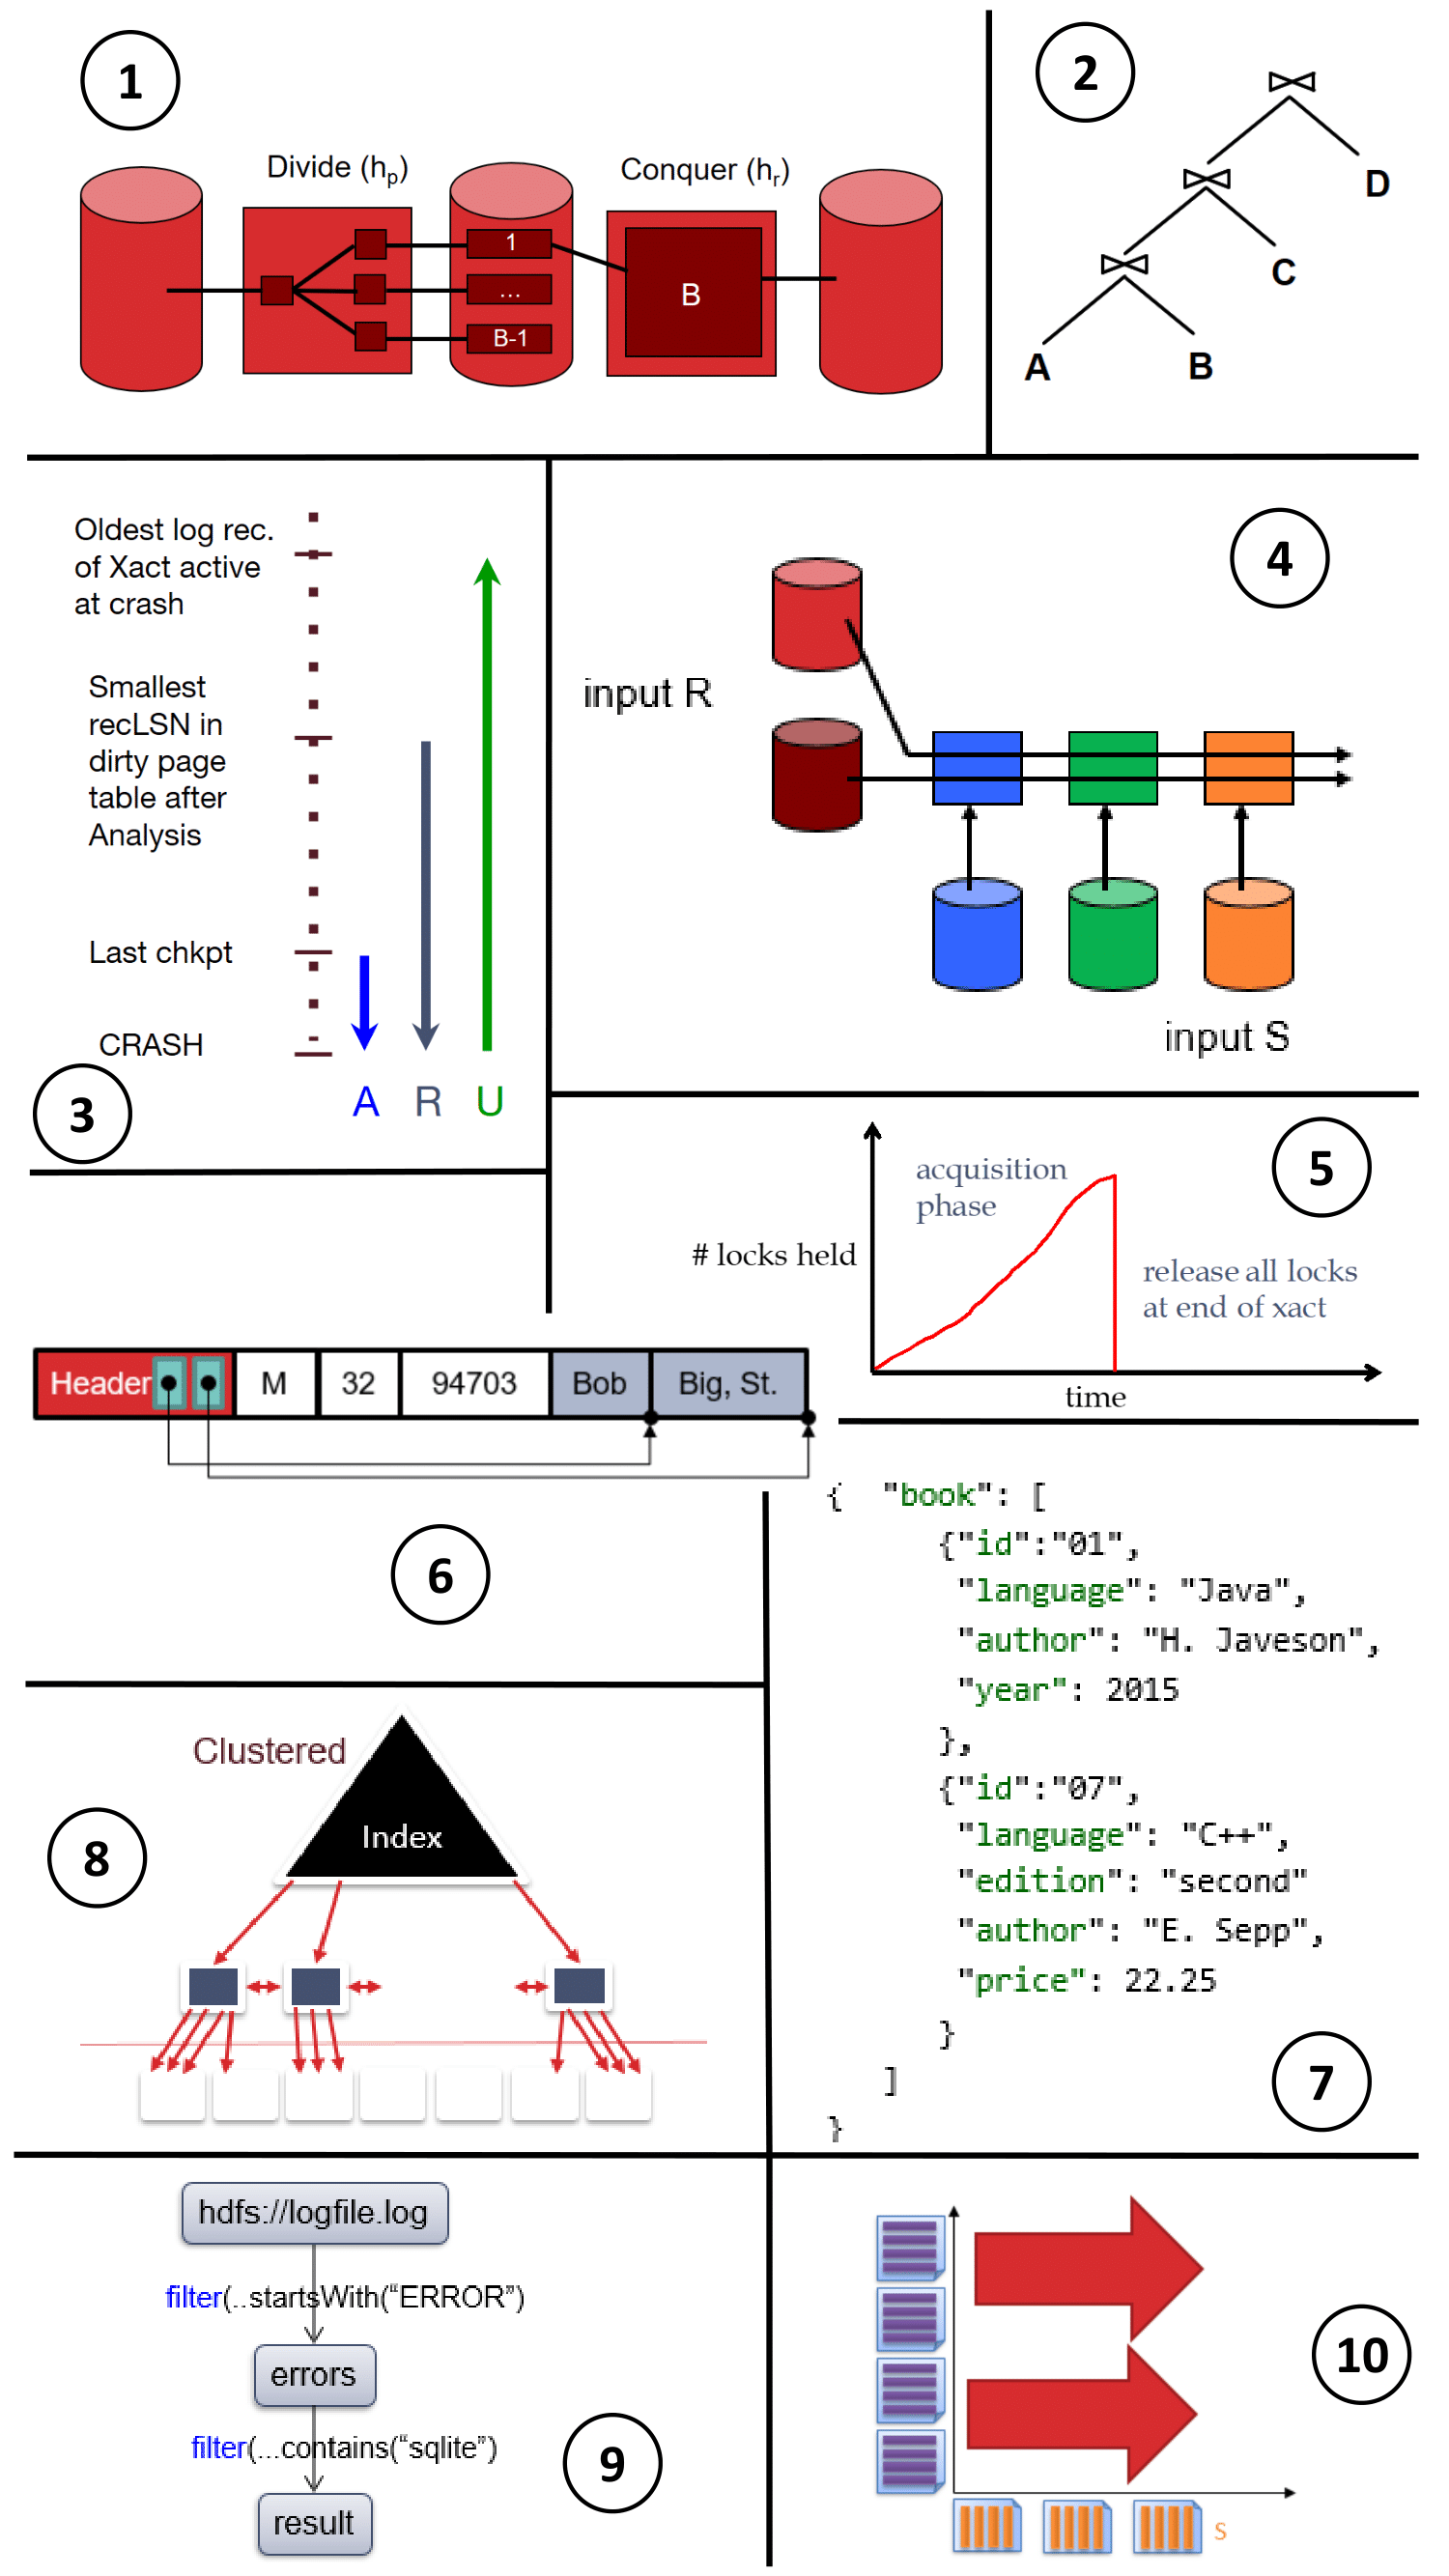
\includegraphics[width=.8\linewidth]{basics.png}
    \caption{Basics of Database.}
    \label{fig1}
\end{figure}
\newpage





\section{SQL and Relational Algebra \textbf{[8 points]}}
\begin{enumerate}
    \item[1.] [\textbf{4 points}] \textbf{SQL} \\
        You want to use your SQL skills to infer what is happening during the Battle of Hogwarts, and you could assume you have the following tables:
        \\
        \\
        CREATE TABLE Wizards(wizid integer, name text, house text, evil boolean, PRIMARY KEY(wizid));
        \\
        \\
        CREATE TABLE Spells(sid integer, name text, offensive boolean, PRIMARY KEY (sid));
        \\
        \\
        CREATE TABLE Attacks(attackid integer, attacker integer, attacked integer, spell integer,\\
        PRIMARY KEY (attackid), FOREIGN KEY(spell) REFERENCES Spells,\\
        FOREIGN KEY(attacker) REFERENCES Wizards, FOREIGN KEY(attacked) REFERENCES Wizards);
        \\
        \\
        \textbf{Note}: For all of the following questions, you do not need any Harry Potter knowledge. Any understanding of Wizards or Spells will not be helpful.
        \begin{enumerate}
            \item[(a)] [\textbf{2 points}] Select all of the following queries that return the name of each wizard who has been an
                attacker more than 3 times. Do not assume that names are unique.\\
                \begin{enumerate}
                    \item[(A)] SELECT name FROM Wizards, Attacks\\
                        WHERE wizid = attacker\\
                        GROUP BY attacker, name\\
                        HAVING COUNT(*) \textgreater  3;\\
                    \item[(B)] SELECT name FROM Wizards, Attacks\\
                        WHERE wizid = attacker\\
                        GROUP BY name\\
                        HAVING COUNT(*) \textgreater 3;\\
                    \item[(C)] SELECT name FROM\\
                        \quad (SELECT name FROM Wizards, Attacks\\
                        \quad\quad WHERE wizid = attacker) AS a\\
                        GROUP BY attacker,name\\
                        HAVING COUNT(*) \textgreater 3\\
                        ORDER BY COUNT(name);\\
                        \\
                \end{enumerate}
            \item[(b)] [\textbf{2 points}] Select all of the following queries that return the name of all of the spells that have never
                been used in an attack.\\
                \begin{enumerate}
                    \item[(A)] SELECT name\\
                        FROM Spells\\
                        WHERE sid NOT IN\\
                        (SELECT spell FROM Attacks);\\
                    \item[(B)] SELECT name\\
                        FROM Spells\\
                        WHERE NOT EXISTS\\
                        (SELECT * FROM Attacks WHERE spell = sid);\\
                    \item[(C)] SELECT Spells.name\\
                        FROM Spells, Wizards, Attacks\\
                        WHERE wizid = attacker and spell = sid;\\ \\ \\ \\ \\ \\
                \end{enumerate}
        \end{enumerate}

        \item[2.][\textbf{4 points}] \textbf{Relational Algebra} \\
        Consider two relations with the same schema: R(A,B,C) and S(A,B,C). Which one of the following relational
        algebra expressions is not equivalent to the others?
        \begin{enumerate}
            \item[(A)] $\pi_{R.A}((R\cup S)-S)$
            \item[(B)] $\pi_{R.A}(R)-\pi_{R.A}(R\cap S)$
            \item[(C)] $\pi_{R.A}(R-S)\cap \pi_{R.A}(R)$
            \item[(D)] $\pi_{R.A}(R-S)$
        \end{enumerate}
\end{enumerate}





\newpage
\section{B+ Trees \textbf{[8 points]}}
Given the following (degree d = 1) B+ tree:
\begin{figure}[h]\centering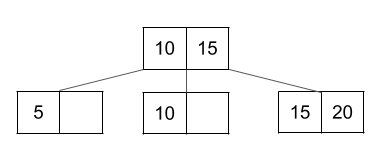
\includegraphics[height=3cm]{b+tree.png}\end{figure}\\
\begin{enumerate}
    \item[1. ] [\textbf{4 points}]  Draw what the tree looks like after adding 2, 6, and 12 in that order.\\ \\ \\ \\ \\ \\ \\ \\ \\ \\ \\
    \item[2.] [\textbf{4 points}]
        \noindent For the following questions, consider the tree directly after 2, 6, and 12 have been added.
        \begin{enumerate}
            \item[(a)] [\textbf{2 points}] What is the maximum number of inserts we can do without changing the height of the tree?\\ \\ \\
                \item[(b)][\textbf{2 points}] What is the minimum number of inserts we can do that will change the height of the tree?\\ \\ \\ \\ \\ \\
        \end{enumerate}
\end{enumerate}






\newpage
\section{Buffer Management \textbf{[8 points]}}
We’re given a buffer pool with 4 pages, which is empty to begin with. Answer the following questions given
this access pattern:
\begin{center}
    A B C D E B A D C A E C 
\end{center}
\begin{enumerate}
    \item[1.][\textbf{2 points}] What is the hit rate for MRU?\\ \\ \\ \\
    
    \item[2.][\textbf{2 points}] In order of when they were first placed into the buffer pool, what pages remain in the buffer pool after this sequence of accesses?\\ \\ \\ \\ 
    
    \item[3.][\textbf{2 points}] What is the hit rate for CLOCK?\\ \\ \\ \\ \\ \\
    
    \item[4.][\textbf{2 points}] Which pages are in the buffer pool after this sequence of accesses?\\ \\ \\ \\ \\ \\
\end{enumerate}






\newpage
\section{External Sorting and Hashing \textbf{[10 points]}}
\begin{enumerate}
    \item[1.] [\textbf{5 points}] Let’s Sort and Hash This Out!
        \\
        \\
        Now you're facing the problem of figuring out the steps to sort a table in your DBMS. Assume your table is 100 pages and you have 5 buffer pages in memory. Please fill out the following pass-by-pass guide that details the number and the length of runs created after each pass in External Merge Sort.
        \\
        \\
        In the \textbf{second} blank for each pass, write all unique run lengths in \textbf{increasing} order, separated by commas. In the \textbf{first} blank for each pass, write the number of runs corresponding to each run length specified in the second blank, separated by commas.\\ \\
        For example, if there were 3 runs of length 50 created after Pass 0, then write 3 for the first blank and 50
        for the second blank on the line for Pass 0.
        If instead there were 6 runs created in total: 2 runs of length 10, 1 run of length 25, and 3 runs of length
        50, then write 2, 1, 3 for the first blank and 10, 25, 50 for the second blank. \\ \\
        If the algorithm terminates before the last pass, write 0 for all blanks in unused passes. \\
        \begin{enumerate}
            \item[(a)][\textbf{3 points}] Fill out the numbers for each blank in the following passes.\\
            \begin{itemize}
                \item Pass 0: \underline{\quad\quad\quad\quad} run(s) of \underline{\quad\quad\quad\quad} page(s) are created.\\
                \item Pass 1: \underline{\quad\quad\quad\quad} run(s) of \underline{\quad\quad\quad\quad} page(s) are created.\\
                \item Pass 2: \underline{\quad\quad\quad\quad} run(s) of \underline{\quad\quad\quad\quad} page(s) are created.\\
                \item Pass 3: \underline{\quad\quad\quad\quad} run(s) of \underline{\quad\quad\quad\quad} page(s) are created.\\
                      %            \item Pass 4: \underline{\quad\quad\quad\quad} run(s) of \underline{\quad\quad\quad\quad} page(s) are created.\\ \\
            \end{itemize}
            \item[(b)][\textbf{2 points}] Based on the guide, how many I/Os does the entire External Sort on this table take?
            \\
            \\
            \\
            \\
            \\
        \end{enumerate}

    \item[2.] [\textbf{5 points}] Now you also want to hash the table
        which requires an exhaustive of the hashing process as well. Still assuming the table is 100 pages and you have 5 buffer pages in memory, please fill out the following guide which details the number and size of partitions created after each partitioning pass in External Hashing. You could assume uniform hash functions are used in each pass.\\ \\
        In the \textbf{first} blank for each pass, write the total number of partitions created after the pass. In the \textbf{second}
        blank, write the number of pages in each of those partitions. If not all partition passes are needed, write 0
        for all blanks in unneeded passes.\\ \\
        \begin{enumerate}
            \item[(a)][\textbf{3 points}] Fill out the numbers for each blank in the following passes. \\
            \begin{itemize}
                \item Partitioning Pass 1: \underline{\quad\quad\quad\quad} partition(s) of \underline{\quad\quad\quad\quad} page(s) are created.\\
                \item Partitioning Pass 2: \underline{\quad\quad\quad\quad} partition(s) of \underline{\quad\quad\quad\quad} page(s) are created.\\
                \item Partitioning Pass 3: \underline{\quad\quad\quad\quad} partition(s) of \underline{\quad\quad\quad\quad} page(s) are created.\\
                \item Partitioning Pass 4: \underline{\quad\quad\quad\quad} partition(s) of \underline{\quad\quad\quad\quad} page(s) are created.\\
                      %           \item Partitioning Pass 5: \underline{\quad\quad\quad\quad} partition(s) of \underline{\quad\quad\quad\quad} page(s) are created.\\ \\
            \end{itemize}
            \item[(b)][\textbf{2 points}] Based on the guide, how many I/Os does the entire External Hashing process on this table
            take? Remember that External Hashing consists of both the divide phase and the conquer phase.
            \\
            \\
            \\
            \\
            \\
        \end{enumerate}
\end{enumerate}



\newpage
\section{Join Algorithms \textbf{[8 points]}}
There are two tables: Candies and Stores. \\

Candies(cid int, cname text, manufacturer text) \\

Stores(sid int, sname text, cid int) \\
\\
You want to see which stores carry your favorite candies, but you are unsure of which join
algorithm you should utilize to perform the query below.
\begin{verbatim}
SELECT C.cid, COUNT(*)
FROM Candies C, Stores S
WHERE C.cid = S.cid
GROUP BY C.cid;
\end{verbatim}

\noindent
We have 100 pages of Candies and 60 pages of Stores. The Candies table has 5 records per
page, and the Stores table has 10 records per page. Be sure to choose the inner and outer relations such that you minimize the I/O cost. You have 25 buffer pages at your disposal.


\begin{enumerate}
    \item \textbf{[2 points]}
          What is the I/O cost of a block nested loops join between Candies and Stores? \\ \\ \\ \\
    \item \textbf{[2 points]}
          What is the I/O cost of an index nested loops join between Candies and Stores?
          (There is an index on Stores.cid, and it takes an average of 3 I/O's to find a matching tuple.) \\ \\ \\ \\
    \item \textbf{[2 points]}
          What is the I/O cost of a sort-merge join between Candies and Stores? \\ \\ \\ \\
    \item \textbf{[2 points]}
          What is the I/O cost of a grace hash join between Candies and Stores?
          (Assume we have hash functions that can partition the data evenly.)
\end{enumerate}
%\textbf{Your answer:}





\newpage

\section{Query Optimization  \textbf{[10 points]}}
Assume the following:
\begin{itemize}
    \item Column values are uniformly distributed and independent from one another
    \item Use System R defaults (1/10) when selectivity estimation is not possible
    \item Primary key IDs are sequential, starting from 1
    \item Our optimizer \textbf{does not consider interesting orders}
\end{itemize}
We have the following schema:
% \\
% Consider three relations Student(sid, b) and S(a), with 1000 tuples and 500 tuples respectively. We have
% an index on R.a with 50 unique integer values uniformly distributed in the range [1, 50], and an index on
% S.a with 25 unique integer values uniformly distributed in the range [1, 25]. We do not have an
% index on R.b.\\
\begin{figure}[h]\centering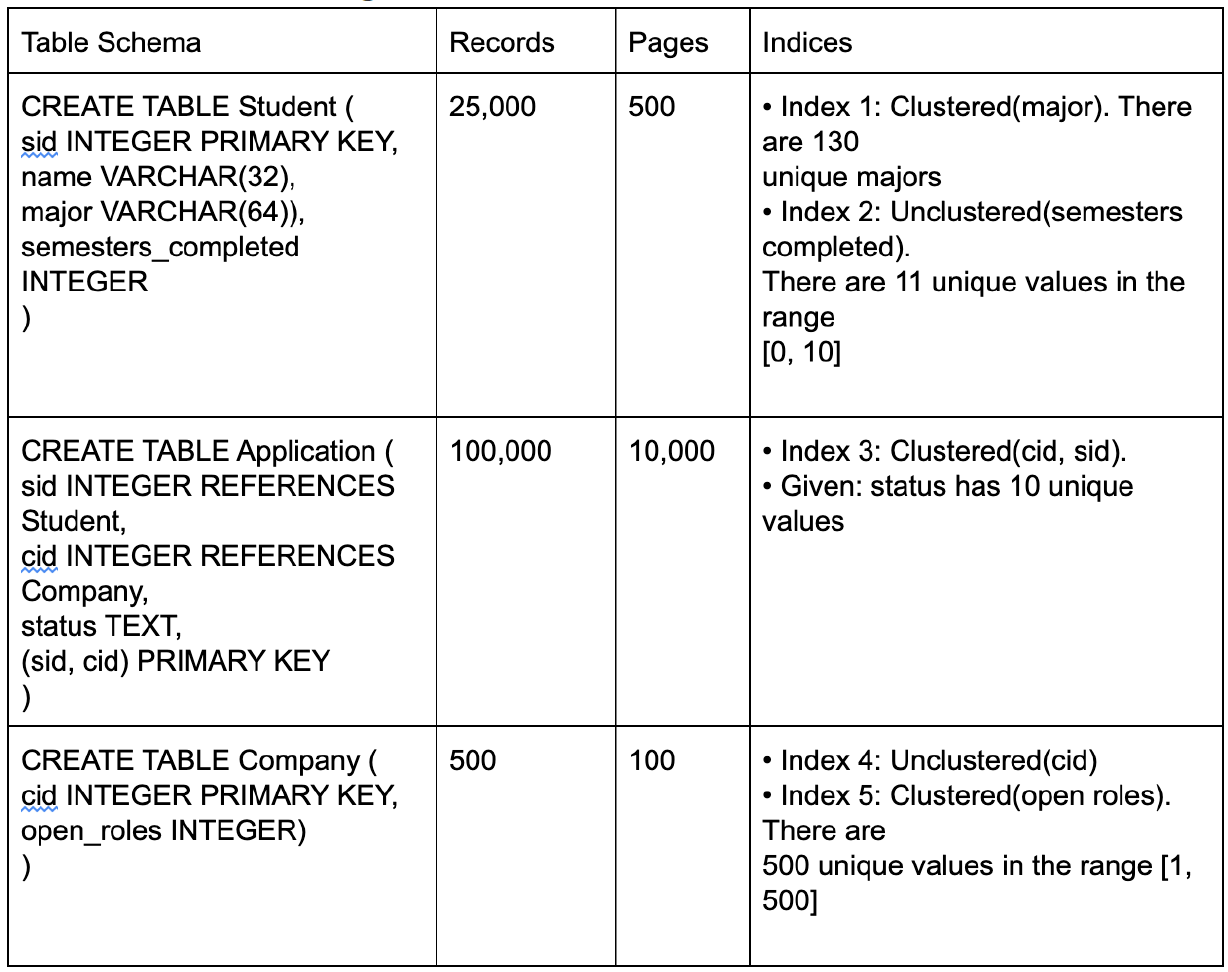
\includegraphics[height=10cm]{query_opt.png}\end{figure}\\
Consider the following query:\\ \\
SELECT Student.name, Company.open\_roles, Application.referral\\
FROM Student, Application, Company\\
WHERE Student.sid = Application.sid \hfill -- (Selectivity 1)\\
% AND Application.cid = Company.cid  \hfill -- (Selectivity 2)\\
AND Student.semesters\_completed $>$ 4 \hfill -- (Selectivity 2)\\
AND (Student.major='CS' OR Company.open\_roles $<=$ 50) \hfill -- (Selectivity 3)\\
% AND NOT Application.status = 'limbo' \hfill -- (Selectivity 4)\\
ORDER BY Company.open\_roles;
\begin{enumerate}
    \item[1.] [\textbf{4 points}] For the following questions, calculate the selectivity of each of the labeled Selectivities above.
        \begin{enumerate}
            % \item Selectivity 1 \\ \\
            \item Selectivity 2 \\ \\ \\ \\
            \item Selectivity 3 \\ \\ \\ \\
        \end{enumerate}
    \item[2.] [\textbf{6 points}] For each predicate, which pass is the first one of Selinger's algorithm that uses its selectivity to estimate output size? (\textbf{Pass 1, 2 or 3}?)
        \begin{enumerate}
            \item Selectivity 1: \\
                  $\square$ Pass 1 \quad $\square$ Pass 2 \quad $\square$ Pass 3 \\
                  % \item Selectivity 2 \\
                  % $\square$ Pass 1 \quad $\square$ Pass 2 \quad $\square$ Pass 3
            \item Selectivity 2 \\
                  $\square$ Pass 1 \quad $\square$ Pass 2 \quad $\square$ Pass 3 \\
            \item Selectivity 3 \\
                  $\square$ Pass 1 \quad $\square$ Pass 2 \quad $\square$ Pass 3 \\
                  % \item Selectivity 5 \\
                  % $\square$ Pass 1 \quad $\square$ Pass 2 \quad $\square$ Pass 3
        \end{enumerate}
\end{enumerate}




\newpage
\section{Concurrency Control and Lock Manager \textbf{[8 points]}}
\begin{enumerate}
    \item[1.] \textbf{[4 points]} \textbf{Concurrency Control} \\
        Consider the following schedule
        \begin{figure}[h]
            \centering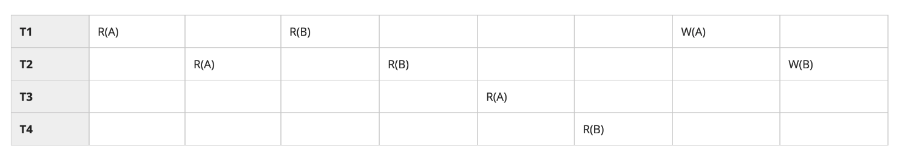
\includegraphics[height=3.2cm]{conflict.png}
        \end{figure}
        \begin{enumerate}
            \item[(a)] \textbf{[2 points]} Draw the conflict dependency graph for the schedule.\\ \\ \\ \\ \\ \\ \\ \\
            \item[(b)] \textbf{[2 points]} Is this schedule conflict serializability? If so, write down all the conflict equivalent serial schedules. If not, explain the reason.  \\ \\ \\ \\ \\ \\ \\
        \end{enumerate}

    \item[2.] \textbf{[4 points]} \textbf{Lock Manager} \\
        Given the database system shown below:
        \begin{figure}[ht]
            \centering
            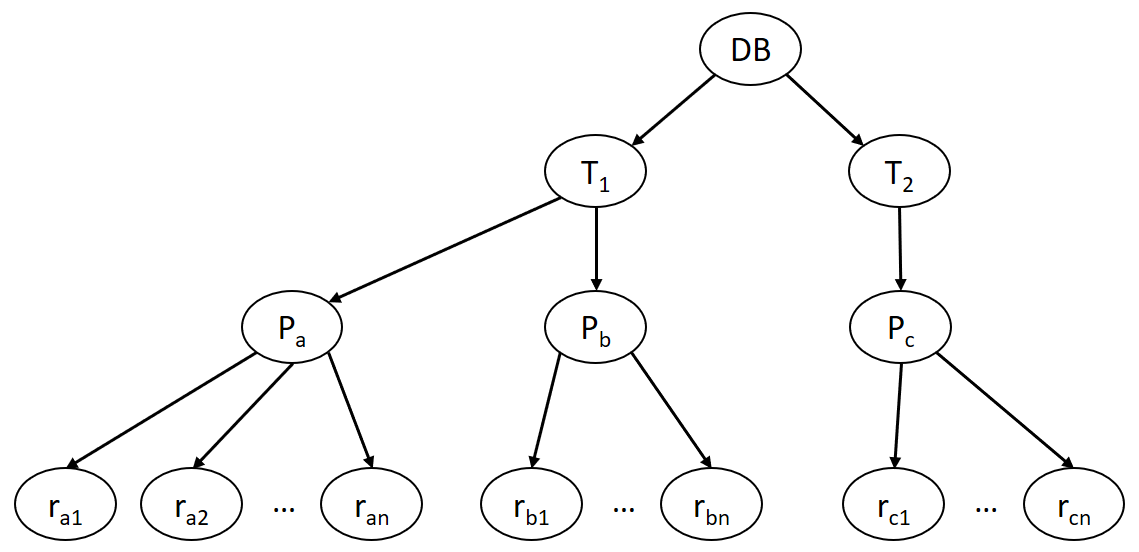
\includegraphics[width=0.7\linewidth]{lock_mode}
        \end{figure}
        \begin{itemize}
            \item[(a)] \textbf{[2 points]} Which lock modes (including S, X, IS, IX, or SIX) on which resources are necessary to modify $P_a$? \\
            \item[(b)] \textbf{[2 points]} Which lock modes (including S, X, IS, IX, or SIX) held by other transactions on $P_a$ would prevent us from reading $r_{a1}$? \\
        \end{itemize}
\end{enumerate}





\newpage
\section{Recovery \textbf{[9 points]}}
\begin{enumerate}
    \item[1.] \textbf{[3 points]} For the following statements, please answer whether it is True or False.
        \begin{enumerate}
            \item When a transaction commits, any modified buffer pages must be written to durable storage.\\ \\
            \item When aborting a transaction, it may be necessary to modify pages on disk.\\ \\
            \item During recovery, the ARIES protocol may redo aborted transactions.\\ \\
            \item The pageLSN contains the LSN of the last operation to modify the page.\\ \\
            \item The tail of the log is always flushed after every update operation.\\ \\
            \item A system that uses a FORCE, STEAL policy does not need to undo any operations after a crash.\\ \\
            \item The recovery manager is responsible for Atomicity and Durability, as defined by the ACID acronym.\\ \\
            \item During a transaction abort, we redo all updates made by the transaction.\\ \\ \\ \\ \\ \\
        \end{enumerate}

    \item[2.] \textbf{[6 points]} Consider the following log.
        Some of the records have been omitted.
        The system crashes immediately after LSN 100 and begins recovery.
        During analysis, we recreate the transaction table and dirty page table shown below.
        \begin{figure}[ht]
            \centering
            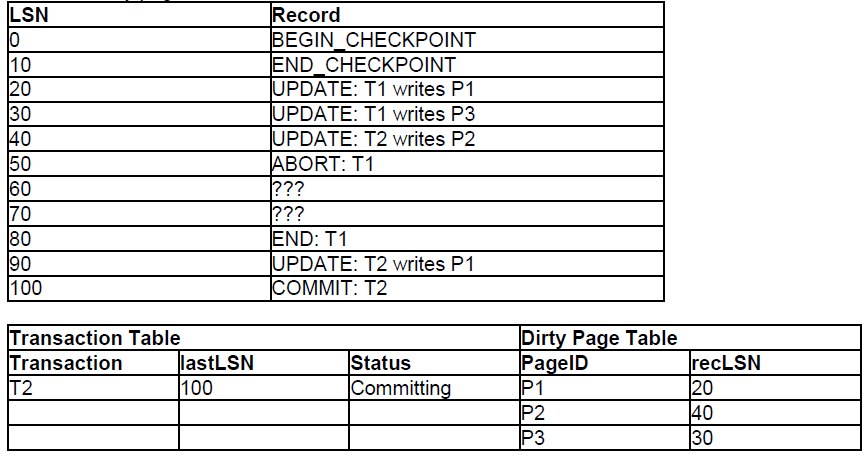
\includegraphics[width=0.9\linewidth]{recovery}
        \end{figure}
        \begin{enumerate}
            \item\textbf{[2 points]} What are the missing log records (??? in the image above)?  \\ \\ \\ \\
            \item\textbf{[2 points]} Which LSN should the REDO phase start on? \\ \\ \\ \\
            \item\textbf{[2 points]} What will be written during the UNDO phase? \\ \\ \\ \\
        \end{enumerate}
\end{enumerate}




\newpage
\section{Database Design \textbf[9 points]}

\begin{enumerate}
    \item[1.] \textbf{[3 points]} \textbf{ER Model} \\
        Suppose that you are tasked with designing a new final exam scheduling system to make it
        easier on students. Using the following assumptions, fill in the ER diagram we give you.
        \begin{itemize}
            \item A student may take any number of exams, and every exam is taken by at least one student.
            \item An exam is uniquely identified by the combination of a course and a semester.
            \item Every exam has at least one supervisor. A supervisor oversees exactly one exam.
            \item There is at least one question on every exam, and a question appears on at most one exam.
            \item A question on an exam may be answered by any number of students, and a student may answer any number of questions on an exam.
        \end{itemize}
        \begin{figure}[ht]
            \centering
            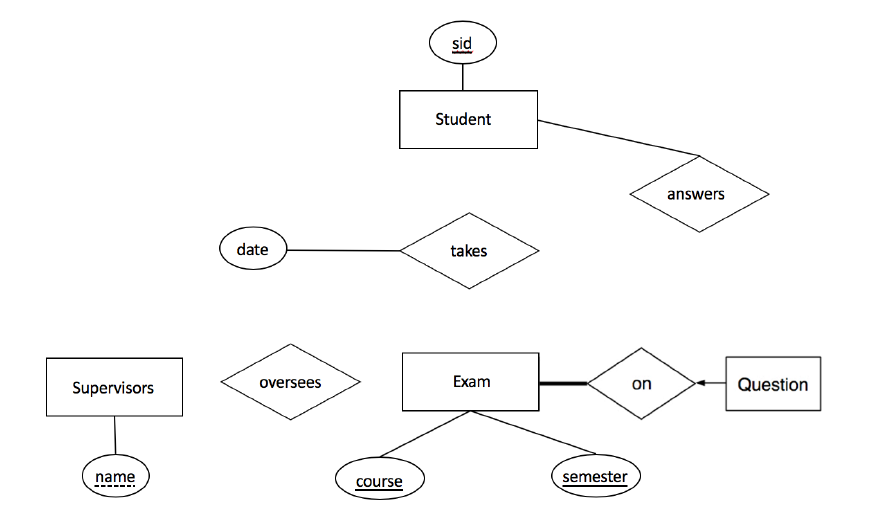
\includegraphics[width=0.85\linewidth]{er_model}
        \end{figure}
        Given three types of edges (\textbf{Bold Arrow}, \textbf{Bold Line} and \textbf{Thin Line}), answer the following questions
        \begin{enumerate}
            \item\textbf{[1 point]} What type of edge should be drawn between the Supervisors entity and the oversees relationship set? \\ \\ \\ \\
            \item\textbf{[1 point]} What type of edge should be drawn between the Exam entity and the oversees relationship set? \\ \\ \\ \\
            \item\textbf{[1 point]} What type of edge should be drawn between the Student entity and the takes relationship set? \\ \\ \\ \\
            %    \item\textbf{[1 point]} What type of edge should be drawn between the Exam entity and the takes relationship set? \\ \\ \\ \\
            %    \item\textbf{[1 point]} What type of edge should be drawn between the Questions entity and the answers relationship set? \\ \\ \\ \\
        \end{enumerate}

    \item[2.]  \textbf{[3 points]} \textbf{Functional Dependencies} \\
        We have a relation R(A, B, C, D, E). We are told that the set of functional dependencies is
        F = {E → BC, A → B, C → D, AD → C}.
        \begin{itemize}
            \item[(a)] \textbf{[1 point]} What is E+? \\ \\ \\ \\
            \item[(b)] \textbf{[1 point]} Is the attribute set ACE the superkey for relation R? \\ \\ \\ \\
            \item[(c)] \textbf{[1 point]} Is relation R already in Boyce-Codd Normal Form (BCNF)? \\ \\ \\ \\
        \end{itemize}

    \item[3.] \textbf{[3 points]} \textbf{Normalization and Decomposition} \\
        Decompose $R=ABCDEFGH$ into BCNF in the order of the given functional dependencies: $F=\{ C\rightarrow A, B\rightarrow EF, H\rightarrow BCG, F\rightarrow CD, G\rightarrow B\}$.\\
        Select all the following tables included in the final decomposition.
        \begin{enumerate}
            \item[(A)] $AC$ \\
            \item[(B)] $BCDGH$ \\
            \item[(C)] $BCGH$ \\
            \item[(D)] $BG$ \\
            \item[(E)] $DH$ \\ \\ \\ \\
        \end{enumerate}
\end{enumerate}




\newpage
\section{Parallel Query Processing \textbf{[8 points]}}
\begin{enumerate}
    \item \textbf{[2 points]} \textbf{Partition} \\
          Suppose we have a table of 1200 rows, perfectly range-partitioned across 2 machines in order.\\
          We just bought the 3th machine for our database, and we want to run parallel sorting using all 3 machines.\\
          The first step in parallel sorting is to re-partition the data across all 3 machines, using range partitioning. (The new machine will get the last range.)\\
          For each of the first 2 machines, \textbf{how many rows} will it send across the network during the re-partitioning?
          (You can assume the new ranges are also perfectly uniform.) \\ \\ \\ \\
    \item \textbf{[6 points]} \textbf{Parallel Algorithm} \\
          Assume that we have a 100 page table R that we will join with a 400 page table S.
          All the pages start on machine 1, and there are 4 machines in total with 30 buffer pages each.
          \begin{itemize}
              \item[(a)] \textbf{[2 points]} How many passes are needed to do a parallel unoptimized Sort-Merge Join (SMJ) on the data? For
                  this question a pass is defined as a full pass over either table (so if we have to do 1 pass over R and 1 pass
                  over S it is 2 total passes). \\ \\ \\ \\
              \item[(b)] \textbf{[2 points]} How many passes are needed to a parallel Grace Hash Join on the data? \\ \\ \\ \\
              \item[(c)] \textbf{[2 points]} We want to calculate the max in parallel using hierarchical aggregation. What value should
                  each machine calculate and what should the coordinator do with those values? \\ \\ \\ \\
          \end{itemize}
\end{enumerate}




\newpage
\section{MapReduce and Data Mining \textbf{[9 points]}}

\begin{enumerate}

    \item \textbf{[2 points]} \textbf{Basics} \\
          Select all the true statement(s): \\ \\
          A. In Distributed File System (DFS), a file system in which large files are partitioned into smaller files,
          and then distributed and replicated several times on different nodes for fault tolerance. \\ \\
          B. Both the Map and Reduce phases can be split among different
          workers on different machines, with workers performing independent tasks in parallel. \\ \\
          C. Since the Reduce phase must wait until the entire Map phase completes, we must restart the entire Map phase if one map task
          fails. \\ \\
          D. The order of the basic KDD (Knowledge Discovery in Database) process is Data Cleaning, Data Selection, Data Mining \& ML, Evaluation. \\  \\
          E. The ultimate goal in machine learning is to find a model that best fits the training data. \\  \\
          F. The $k$-means algorithm is guaranteed to converge to the local optimum. \\ \\
          G. The bag-of-words model encodes the text feature as a vector. \\ \\
          H. A common form of feature engineering on categorical data is one-hot-encoding. \\ \\ \\ \\

    \item \textbf{[7 points]} \textbf{$k$-means} \\
          Use the MapReduce implementation of the $k$-means algorithm to cluster the following 8 data points:
          \begin{align*}
              x_1 & = (2,10), \ x_2 = (2,5), \ x_3 = (8,4), \ x_4 = (5,8), \\
              x_5 & = (7,5),  \ x_6 = (6,4), \ x_7 = (1,2), \ x_8 = (4,9).
          \end{align*}
          Suppose the number of clusters is 3, and the initial cluster centers are $x_1$, $x_4$ and $x_7$.
          \begin{itemize}
              \item[(a)] \textbf{[2 points]} What is the input of the Reduce function in the first iteration. \\ \\ \\ \\
              \item[(b)] \textbf{[2 points]} What is the output of the Reduce function in the first iteration. \\ \\ \\ \\
              \item[(c)] \textbf{[3 points]} How many more iterations are needed to converge? Draw the result for each iteration. \\ \\ \\ \\
          \end{itemize}

\end{enumerate}




\end{document}

